\lab{Obstacle Avoidance}{Obstacle Avoidance}
\label{lab:ObstacleAvoidance}
\labdependencies{IVPBVPIntro}

\objective{Solve boundary value problems that arise when using Pontryagin's Maximum principle.}

\section*{Pontryagin's Maximum Principle}
Now that we understand how to solve boundary value problems, we can apply this to solve optimal control problems.
Pontryagin's Maximum Principle is a very common way to formulate control problems as BVPs.

\subsection*{Fixed Time, Fixed Endpoint}
We will begin with the more simple fixed time horizon problems.
Fixed time horizon problems are commonly reformulated as boundary value problems, and we can apply what we have already learned about solving BVPs to make these problems easier to solve.
We introduce fixed time horizon problems with a cost functional of the following form
\begin{equation}
    J(u) = \int_{t_0}^{t_f}L(t,s(t),u(t))dt + K(t_f,s_f),
\end{equation}
where $t_0$ and $t_f$ are fixed.
In this functional, $L(t,s(t),u(t))$ represents the cost of a certain path determined by the control $u$, and $K(t_f,s_f)$ is the terminal cost.
We also have that
\begin{equation}\label{eq:state_ode}
    \dot{s} = f(t,s,u),\; s_0 = s(t_0),\; s_f = s(t_f).
\end{equation}
In these equations $t$ is time, $s$ is the state variable, and $u$ is the control variable.
The maximum principle also uses the Hamiltonian equation
\begin{equation}
    H(t,s,u,p) = \langle p,f(t,s,u)\rangle - L(t,s,u),
\end{equation}
where $p$ is a newly introduced variable called the costate.
This Hamiltonian is then used to define an ODE system.
This first equation defines a costate ODE system
\begin{equation}\label{eq:costate_ode}
    \dot{p}^* = -H_s(t,s^*,u^*,p^*),
\end{equation}
where a variable marked with an asterisk is the optimal choice of that variable, meaning that equation \ref{eq:costate_ode} is only true for the optimal state $s^*$, costate $p^*$, and control $u^*$ functions.
This next equation will allow us to solve for the control in terms of the state and costate
\begin{equation}\label{eq:control_relation}
    0 = H_u(t,s^*,u^*,p^*), \quad \forall t\in[t_0,t_f].
\end{equation}
The combination of these equations will allow us to create a BVP that will solve for the optimal control $u^*$ and the associated states $s^*$.
Our ODE comes from \ref{eq:state_ode}, \ref{eq:costate_ode}, and \ref{eq:control_relation}, and the boundary values will come from our initial and final conditions on $s$.

\subsection*{A Specific Example}
Let 
\begin{align*}
	J(u) &= \int_0^{30} x^2 + \frac{2\pi}{5}u^2dt,\\
	\dot{s} &=  \begin{bmatrix}x'\\u \end{bmatrix}, \text{ and } x''=u.
\end{align*}
Then
\begin{align*}
	\begin{split}
	H(t,s,u,p) &= \langle p,f(t,s,u)\rangle - L(t,s,u)\\
	&= \boldsymbol{p} \cdot \dot{\boldsymbol{s}} - x^2 - \frac{2\pi}{5}u^2\\
	&= \boldsymbol{p} \cdot \begin{bmatrix}x'\\u \end{bmatrix} - x^2 - \frac{2\pi}{5}u^2\\
	&= p_1x' + p_2u - x^2 - \frac{2\pi}{5}u^2.
	\end{split}
\end{align*}
We now need to find
\begin{align*}
	H_{\boldsymbol{s}} &= \begin{bmatrix}H_{s_1}\\H_{s_2}\end{bmatrix} = \begin{bmatrix}H_{x}\\H_{x'}\end{bmatrix} = \begin{bmatrix}-2x\\p_1\end{bmatrix},
\end{align*}
and we see that
\begin{align*}
	\boldsymbol{p}' &= \left( \begin{bmatrix}p_1\\p_2\end{bmatrix} \right)'= -H_{\boldsymbol{s}} = \begin{bmatrix}2x\\-p_1\end{bmatrix}.
\end{align*}
Also, we know that $H_u=0$ at the optimal solution, so
\begin{align*}
	H_u &= p_2 - \frac{4\pi}{5}u=0 \Rightarrow u=\frac{5}{4\pi}p_2.
\end{align*}
Thus, we have that
\begin{equation}\label{eq:prob1_ode}
	\left( \begin{bmatrix}x\\x'\\p_1\\p_2\end{bmatrix} \right)' = \begin{bmatrix}x'\\u\\2x\\-p_1\end{bmatrix} = \begin{bmatrix}x'\\ \frac{5}{4\pi}p_2\\2x\\-p_1\end{bmatrix}.
\end{equation}
You will now implement this in problem \ref{prob:obstacle:bvp1}.

\begin{problem}
\label{prob:obstacle:bvp1}
Given the following cost functional and boundary conditions, use the system of ODEs found in \ref{eq:prob1_ode} to solve for and plot the optimal path (position as a function of time, $x(t)$) and acceleration (control as a function of time, $u(t)=\ddot x(t)$).
\begin{align*}
    J(u) &= \int_0^{30} x^2 + \frac{2\pi}{5}u^2dt \\
    s(t) &= \begin{bmatrix}x(t)\\x'(t) \end{bmatrix}, s(0) = \begin{bmatrix}0\\1 \end{bmatrix}, \quad s(30) = \begin{bmatrix}16\\10 \end{bmatrix}
\end{align*}
Plot your solutions for the optimal $x(t)$ (position) and $u(t)$ (acceleration) .
\end{problem}

\begin{figure}[H]
    \centering
    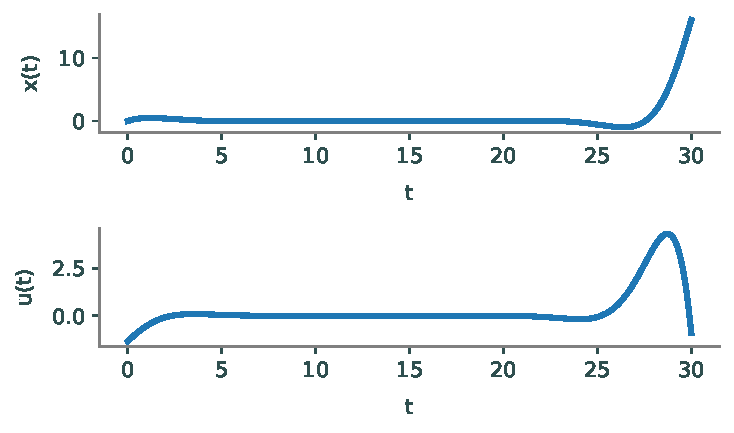
\includegraphics[width=\textwidth]{figures/OA_prob1.pdf}
    \caption{Solution to problem \ref{prob:obstacle:bvp1}}
    \label{fig:OA_prob1}
\end{figure}

\subsection*{Avoiding Collision}
We now expand upon the technique learned above by adding an obstacle in our path.
One area of application that relies heavily on optimal control is autonomous driving.
A common problem in autonomous driving is the avoidance of obstacles.
In this section we will outline a naïve solution to obstacle avoidance with a fixed time horizon.

First we can begin by defining our state variable $s$.
We will want to understand the position and velocity at a given time so we will define the following state variable
\begin{equation}\label{eq:ex-state}
    s(t) = \begin{bmatrix} x(t) \\ y(t) \\ \dot{x}(t) \\ \dot{y}(t) \end{bmatrix} = \begin{bmatrix} s_1(t) \\ s_2(t) \\ s_3(t) \\ s_4(t) \end{bmatrix},
\end{equation}
which allows us to track those states in $\mathbb{R}^2$.

We can then establish the ODE defined in equation \ref{eq:state_ode} by examining $\dot{s}(t)$
\begin{equation*}
    \dot{s}(t) = \begin{bmatrix} \dot{s_1}(t) \\ \dot{s_2}(t) \\ \dot{s_3}(t) \\ \dot{s_4}(t) \end{bmatrix} = \begin{bmatrix} \dot{x}(t) \\ \dot{y}(t) \\ \ddot{x}(t) \\ \ddot{y}(t) \end{bmatrix},
\end{equation*}
and if we define our control $u_1$ and $u_2$ to be acceleration in the $x$ and $y$ directions respectively, then we have
\begin{equation}\label{eq:ex-state-ode}
    \dot{s}(t) = f(t,s,u) = \begin{bmatrix} s_3(t) \\ s_4(t) \\ u_1(t) \\ u_2(t) \end{bmatrix}.
\end{equation}

Next we will define an obstacle.
Since we are using integration to define cost, a reasonable way to model an obstacle in this problem would be to use a function.
It would be helpful if this function is malleable, allowing us to reposition and resize it, based on the needs of the specific situation.
This function also needs to have a large, preferably positive, value in a concentrated location, and it needs to vanish relatively quickly.
A decent selection could be a function based on an ellipse, such as this function
\begin{equation}\label{eq:obstacle}
    C(x,y) = \frac{W_1}{((x-c_x)^2 / r_x + (y - c_y)^2 / r_y)^\lambda + 1}.
\end{equation}
With the function \ref{eq:obstacle} we can manipulate the center by changing $c_x$ and $c_y$, and we can control the size by changing $r_x$ and $r_y$.
Changing the constant $W_1$ allows us to change the relative penalty of occupying the same location as the obstacle, and a reasonable value for $\lambda$ will control the vanishing rate.
We will also include a term in the cost functional that weights against high acceleration.
This will allow us to model the real world more accurately, though the term we will be using is not a perfect representation of real world acceleration limitations.
Our cost functional is the following
\begin{equation}\label{eq:ex-cost-func}
    J(\boldsymbol{u}) = \int_{t_0}^{t_f}1 + C(x(t),y(t)) + W_2\left|\boldsymbol{u}(t)\right|^2 dt,
\end{equation}
where $W_2>0$ defines the relative penalty of high acceleration.
This functional will penalize passing near the obstacle and high levels of acceleration.

With the cost functional defined, we can now create the Hamiltonian and the rest of our BVP.
We get the following Hamiltonian
\begin{equation}\label{eq:ex-Hamiltonian}
    H(t,p,s,u) = p_1s_3 + p_2s_4 + p_3u_1 + p_4u_2 - \left(1 + C(x,y) + W_2\left(u_1(t)^2+u_2(t)^2\right) \right),
\end{equation}
which gives the following costate ODE by equation \ref{eq:costate_ode}
\begin{equation}\label{eq:ex-costate-odes}
    \begin{aligned}
        \dot{p} =
        \begin{bmatrix}
            \dot{p}_1 \\
            \dot{p}_2 \\
            \dot{p}_3 \\
            \dot{p}_4
        \end{bmatrix} =
        \begin{bmatrix}
            C_x(x,y) \\
            C_y(x,y) \\
            -p_1 \\
            -p_2
        \end{bmatrix}.
    \end{aligned}
\end{equation}
Since we're given $H_u = 0$ in equation \ref{eq:control_relation}, then we also have the following relations
\begin{equation}\label{eq:ex-equality-constraints}
    \begin{aligned}
    u_1(t) = \frac{1}{2W_2}p_3(t) \\
    u_2(t) = \frac{1}{2W_2}p_4(t).
    \end{aligned}
\end{equation}


\begin{problem}
\label{prob:obstacle:bvp2}
Using the ODEs found in \ref{eq:ex-state-ode} and \ref{eq:ex-costate-odes}, the obstacle function \ref{eq:obstacle}, and the following boundary conditions and parameters solve for and plot the optimal path.
\begin{align*}
    t_0 = 0 &, \quad t_f = 20\\
    (c_x,c_y) &= (4,1)\\
    (r_x,r_y) &= (5,.5)\\
    \lambda &= 20\\
    s_0 = \begin{bmatrix}6\\1.5\\0\\0 \end{bmatrix}&, \quad s_f = \begin{bmatrix}0\\0\\0\\0 \end{bmatrix}
\end{align*}
You will need to choose a $W_1$ and $W_2$ which allow the solver to find a valid path.
If these parameters are not chosen correctly, the solver may find a path which goes through the obstacle, not around it.
Plot the obstacle using \li{plt.contour()} to be certain path doesn't pass through the obstacle.

Hint: The default for a parameter of \li{solve_bvp()} called \li{max_nodes} is not large enough.
Try at least \li{max_nodes = 30000}.
You may also find it helpful to use the function \li{partial} from the module \li{functools} to preset the parameters for the functions you will be using.
If you are struggling to find viable values for $W_1$ and $W_2$, try $W_1\in (1,40)$ and $W_2\in (0,9)$. 
\end{problem}

\begin{figure}[H]
    \centering
    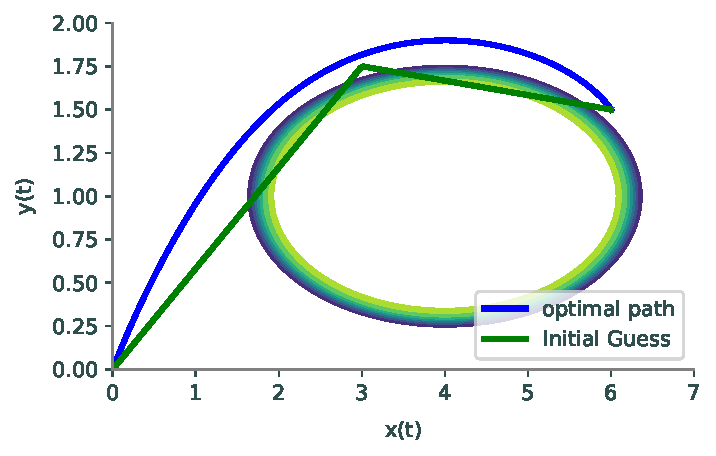
\includegraphics[width=\textwidth]{figures/OA_prob2.pdf}
    \caption{Solution to problem \ref{prob:obstacle:bvp2} for certain choice of parameters.  Here we used $W_1=3$ and $W_2=70$, but those parameters are a choice.  Other choices work, too, but will result in a different optimal path around the obstacle.}
    \label{fig:OA_prob2}
\end{figure}

\section*{Free Time Horizon Problems}
In the previous sections and problems, we were working with BVPs that had a fixed start time $t_0$, and a fixed end time $t_f$.
However, we may also encounter systems that have a free end time.
In order to solve these problems we will need to make some alterations to the problem.
First we will perform a change of basis so that we can work with a fixed end time.
Consider the following system
\begin{align*}
    \dot{x}(t) = f(x(t),t)\quad t\in[0,t_f],
\end{align*}
we can do the following change of basis for the time variable
\begin{align*}
    t &= t_f\hat{t} \\
    \implies \frac{d}{dt} &= \frac{d}{d\hat{t}}\frac{d\hat{t}}{dt} \\
    \implies \frac{d}{dt} &= \frac{d}{d\hat{t}}\frac{1}{t_f}.
\end{align*}
We can now define $z(\hat{t}):=x(t_f\hat{t})$ which gives us the following new system
\begin{align*}
    \dot{z}\left(\hat{t}\right) = t_ff\left(z\left(\hat{t}\right),\hat{t}\right)\quad \hat{t}\in[0,1].
\end{align*}
This system can be solved in the same way we solve the fixed time horizon problems.
But you may notice that we now have an extra unknown parameter, the final time.
Because of this, a free time horizon problem will need one more boundary value to make the system solvable.

Lets now examine an example of a free time horizon problem.
We start with a first-order ODE system. Note that the fixed final time has been replaced with a free final time, and that a needed third boundary condition has been included
\begin{align*}
    \begin{bmatrix}
        y_1\\y_2
    \end{bmatrix}'
    =
    \begin{bmatrix}
        y_2 \\
        cos(t) - 9y_1
    \end{bmatrix},
    \quad y_1(0) = 5/3,\quad y_2(0) = 5,\quad y_1(t_f) = -\frac{5}{3}.
\end{align*}
Now we make the coordinate change, giving the following system
\begin{equation}\label{ex:bvp2}
    \begin{bmatrix}
        z_1\\z_2
    \end{bmatrix}'
    =
    t_f\begin{bmatrix}
        z_2 \\
        \cos(\hat{t}) - 9z_1
    \end{bmatrix},
    \quad z_1(0) = 5/3,\quad z_2(0) = 5,\quad z_1(1) = -\frac{5}{3}.
\end{equation}
Now we can solve this system using \li{solve_bvp} in python.
The new argument \li{p} that we have included in \li{ode()} and \li{bc()} is an \li{ndarray} that contains our parameter $t_f$.

\begin{lstlisting}
def ode(t,y,p):
    ''' define the ode system '''
    return p[0]*np.array([y[1], np.cos(p[0]*t) - 9*y[0]])

def bc(ya,yb,p):
    ''' define the boundary conditions '''
    return np.array([ya[0] - (5/3), ya[1] - 5, yb[0] + 5/3])

# give the time domain
t_steps = 100
t = np.linspace(0,1,t_steps)

# give an initial guess
y0 = np.ones((2,t_steps))
p0 = np.array([6])

# solve the system
sol = solve_bvp(ode, bc, t, y0, p0)
\end{lstlisting}
The attribute \li{sol.p[0]} will give the final time the solver found.

When plotting we need to make sure that we remember that $x(t_f\hat{t}) = z(\hat{t})$, so we plot in the following way
\begin{lstlisting}
plt.plot(sol.p[0]*t,sol.sol(t)[0])
plt.xlabel('t')
plt.ylabel('y(t)')
plt.show()
\end{lstlisting}

\begin{figure}[H]
    \centering
    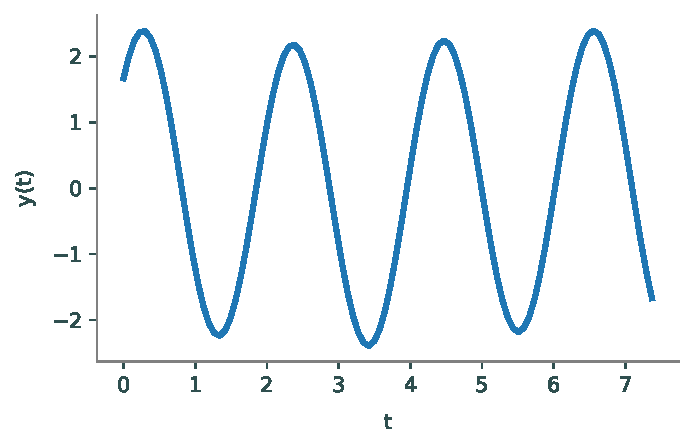
\includegraphics[width=\textwidth]{figures/example2.pdf}
    \caption{The solution to \ref{ex:bvp2}}
\end{figure}

\begin{problem}
\label{prob:obstacle:bvp3}
Solve the following boundary value problem, using $5 \pi$ as the initial guess for \li{p[0]}:
\begin{align*}
    y'' + 3y &= \sin(t)\\
    y(0) = 0,\quad y(t_f) = &\frac{\pi}{2}, \quad y'(t_f) = \frac{1}{2}\left(\sqrt{3}\pi \cot(\pi\sqrt{75}) - 1 \right).
\end{align*}
Plot your solution. What $t_f$ did the solver find?

Hint: Be careful with $\sin(t)$. We have made the substitution for $t$ (it is now scaled by \li{p[0]}).
\end{problem}


\section*{Free Time, Fixed Endpoint Control Problems}

Now that we understand how to formulate free time horizon problems, we can modify our optimal control BVP to become a free time horizon problem.
This is actually the best way to formulate many optimal control problems, as we usually don't know exactly how long it takes to traverse the optimal path. The methodology is exactly the same as we used in the last problem, we only need to find the extra boundary value which will allow us to make the end time a free variable.

To find this extra boundary value we will use the fact that the Hamiltonian is 0 for all $t$ along the optimal path. It is standard to use the final time as the representative so we will assert that
\begin{equation}\label{eq:ex-boundary-value}
    H(t_f,p(t_f),s(t_f),u(t_f)) = 0.
\end{equation}

You may notice that when you solve an optimal control problem as a free end time BVP, the optimal path you get is different than what you found when it was a fixed end time BVP.
This is because the free end time solution actually arrives faster.
The solution found in the fixed end time formulation is the optimal path for a certain fixed end time, but it may not be the overall fastest path that avoids the obstacle.

\begin{problem}
\label{prob:obstacle:bvp4}
Refactor your code from problem \ref{prob:obstacle:bvp2} to create a free end time BVP and use a new boundary value derived from \ref{eq:ex-boundary-value}. Let $W_1 = 4$ and $W_2 = 0.1$, and use $6$ as the initial guess for \li{p[0]}.
Plot the solution you found.
What is the optimal time?
\end{problem}

\begin{figure}[H]
    \centering
    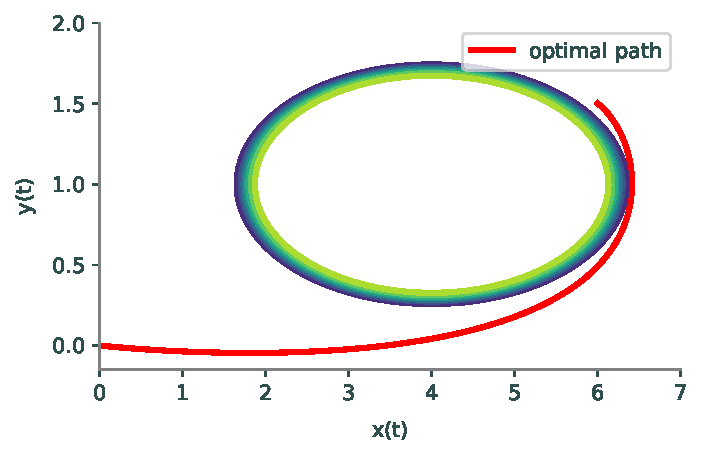
\includegraphics[width=\textwidth]{figures/OA_prob4.pdf}
    \caption{The solution to \ref{prob:obstacle:bvp4}.  Here we used $W_1 = 4$ and $W_2 = 0.1$ and got an optimal time of about 4.47.  Those parameters are a choice.  Other choices work, too, but will result in a different optimal path around the obstacle and in a different optimal time.}
\end{figure}
